
\chapter{Requerimientos}
\section{Introducción}
Para cualquier proyecto de software, es un punto fundamental conocer cuál es la necesidad y el problema que el cliente desea resolver. Para tener una visión holística del problema, se hace necesario definir los requerimientos que satisfagan al cliente y resuelvan el problema.
\newpage

\section{Requerimientos del Cliente}
Se entiende como lo que el cliente espera encontrar cuando interactúe con la aplicación. Bajo la anterior premisa, se definieron los siguientes requerimientos:
\begin{enumerate}
	\item Añadir una tarea.
	\item Añadir subtareas para una tarea.
	\item Añadir un horario universitario.
	\item Añadir un horario de descanso (dormir).
	\item Añadir un horario de transporte.
	\item Añadir una tarea a una materia.
	\item Mostrar todas las tareas pendientes.
	\item Mostrar las tareas pendientes por materia.
	\item Mostrar las tareas pendientes por tipo.
	\item Mostrar las tareas pendientes para una fecha.
	\item Mostrar las tareas pendientes por dificultad.
	\item Mostrar el horario general del usuario.
	\item Mostrar los horarios asignados para las tareas pendientes.
	\item Modificar horario.
	\item Modificar tarea.
	\item Sugerir horarios para realizar tareas.
	\item Sugerir cuánto tiempo podría tomar una tarea.
	\item Sugerir tiempos de pausas activas durante la realización de una tarea.
	\item Alertar de la próxima entrega de una tarea.
	\item Advertir si se debe sacrificar algún espacio de descanso.

\end{enumerate}

\section{Casos de uso}
Los casos de uso describen la interacción del usuario con las diversas funcionalidades planteadas, permitiendo obtener una forma de comunicar los requerimientos de tal forma que sea entendida tanto por usuario como por desarrolladores. Como se podrá observar a continuación, serán cuatro diagramas de caso de uso los que se presentan, donde el motivo por el cual los casos de uso comparten diagrama, es porque se considera que existe cierta relación entre ellos.



\begin{figure}[H]
	\centering
	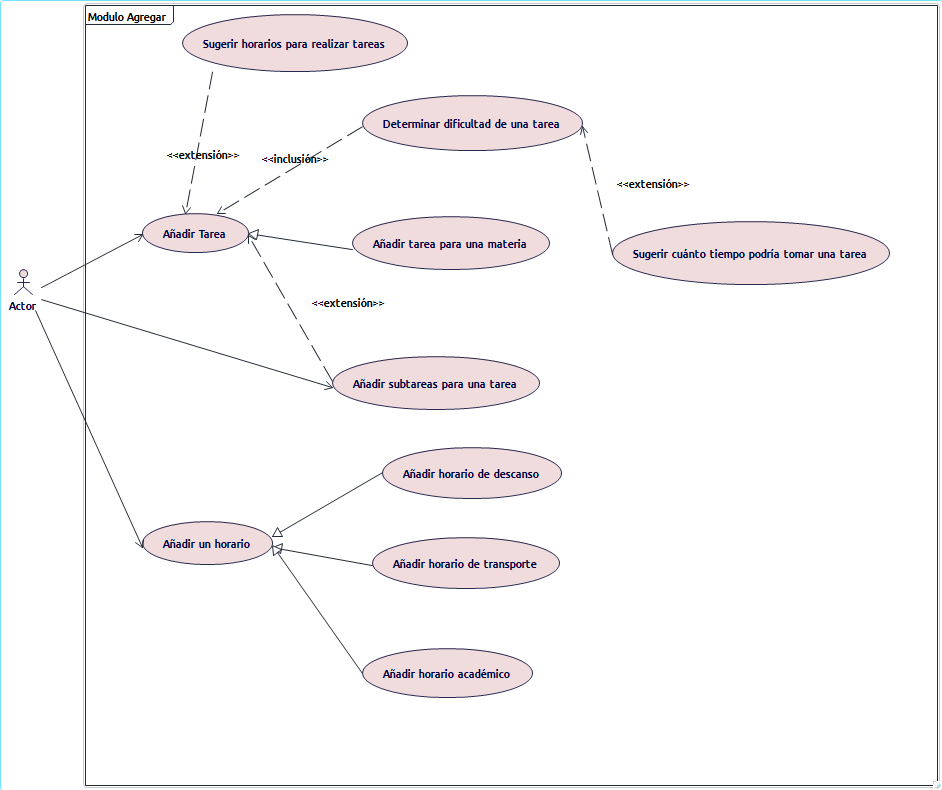
\includegraphics[width=0.7\linewidth]{diseno/requerimientos/imagenes/casouso1}
	\caption{Primer diagrama de caso de uso}
	\label{fig:gantt}
\end{figure}
\begin{figure}[H]
	\centering
	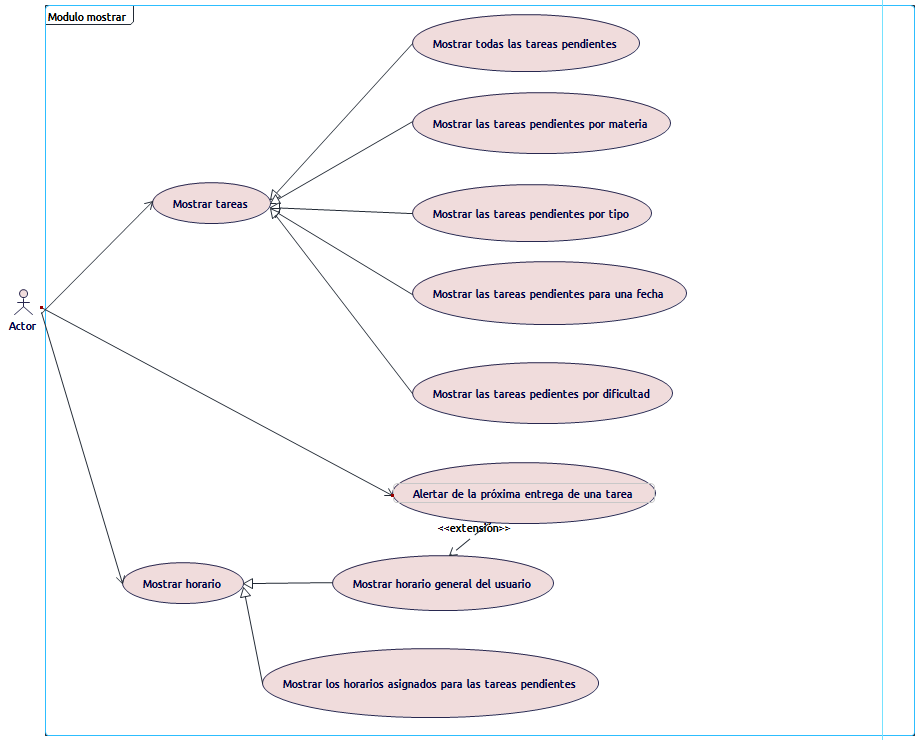
\includegraphics[width=0.7\linewidth]{diseno/requerimientos/imagenes/casouso2}
	\caption{Segundo diagrama de caso de uso}
	\label{fig:gantt}
\end{figure}
\begin{figure}[H]
	\centering
	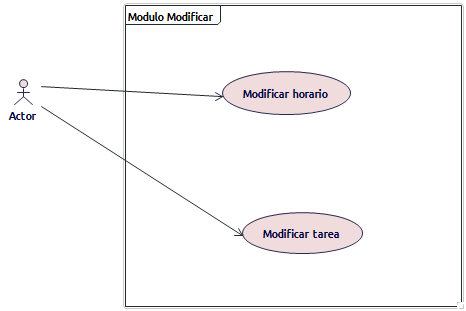
\includegraphics[width=0.7\linewidth]{diseno/requerimientos/imagenes/casouso3}
	\caption{Tercero diagrama de caso de uso}
	\label{fig:gantt}
\end{figure}
\begin{figure}[H]
	\centering
	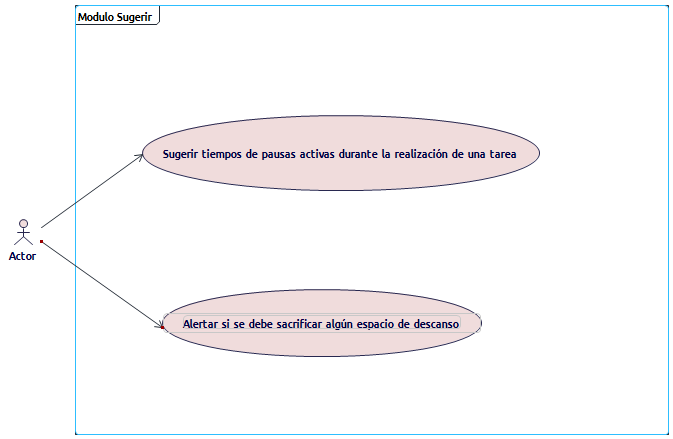
\includegraphics[width=0.7\linewidth]{diseno/requerimientos/imagenes/casouso4}
	\caption{Cuarto diagrama de caso de uso}
	\label{fig:gantt}
\end{figure}

Los diagramas a continuación representan gran importancia complemetando la definición de los requerimientos.

\section{Diagramas de secuencia}
Los diagramas de secuencia permiten obervar la realización del caso de uso, responden el como se va a hacer el requerimiento. Los siguientes son los diagramas de secuencia de 4 casos de uso que se consideran de mayor importancia.

\begin{figure}[H]
	\centering
	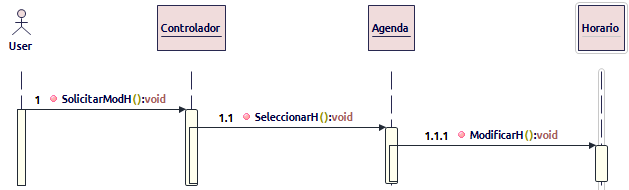
\includegraphics[width=0.7\linewidth]{diseno/requerimientos/imagenes/secuencia1}
	\caption{Diagrama de secuencia caso de uso 14.}
	\label{fig:gantt}
\end{figure}
\begin{figure}[H]
	\centering
	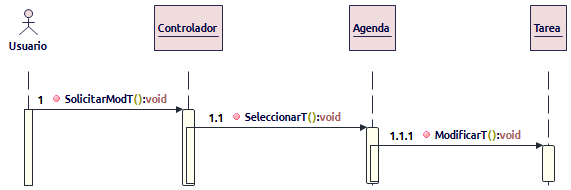
\includegraphics[width=0.7\linewidth]{diseno/requerimientos/imagenes/secuencia2}
	\caption{Diagrama de secuencia caso de uso 15.}
	\label{fig:gantt}
\end{figure}
\begin{figure}[H]
	\centering
	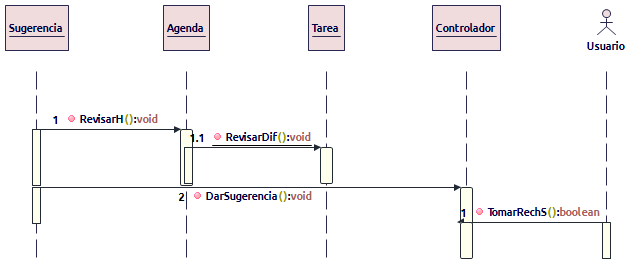
\includegraphics[width=0.7\linewidth]{diseno/requerimientos/imagenes/secuencia3}
	\caption{Diagrama de secuencia caso de uso 16.}
	\label{fig:gantt}
\end{figure}
\begin{figure}[H]
	\centering
	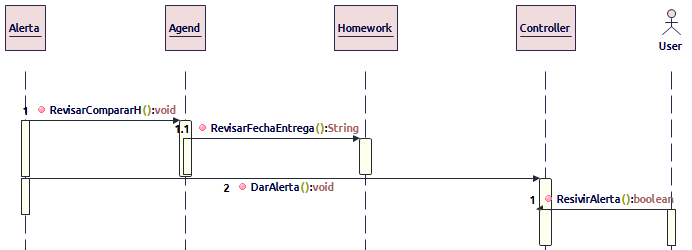
\includegraphics[width=0.7\linewidth]{diseno/requerimientos/imagenes/secuencia4}
	\caption{Diagrama de secuencia caso de uso 19.}
	\label{fig:gantt}
\end{figure}

\section{Diagramas de comunicación}
Igualmente relacionados con los diagramas anteriores, principalmente con el diagrama de secuencia. Su función como su nombre lo indica, consiste en detallar en como se comunican los objetos que solucionan el requerimiento.

Se presentan los diagramas correspondientes a los ya expuestos diagramas de secuencia:

\begin{figure}[H]
	\centering
	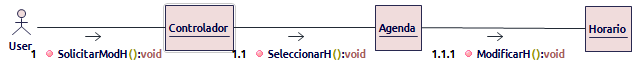
\includegraphics[width=0.7\linewidth]{diseno/requerimientos/imagenes/comunicacion1}
	\caption{Diagrama de comunicación caso de uso 14.}
	\label{fig:gantt}
\end{figure}
\begin{figure}[H]
	\centering
	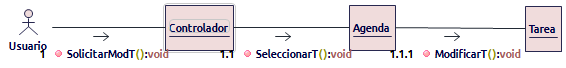
\includegraphics[width=0.7\linewidth]{diseno/requerimientos/imagenes/comunicacion2}
	\caption{Diagrama de comunicación caso de uso 15.}
	\label{fig:gantt}
\end{figure}
\begin{figure}[H]
	\centering
	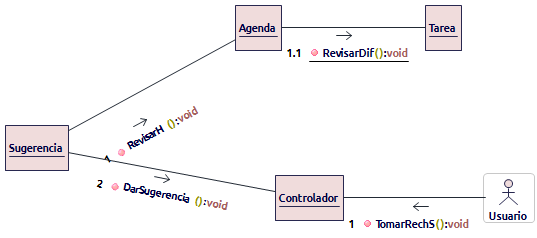
\includegraphics[width=0.7\linewidth]{diseno/requerimientos/imagenes/comunicacion3}
	\caption{Diagrama de comunicación caso de uso 16.}
	\label{fig:gantt}
\end{figure}
\begin{figure}[H]
	\centering
	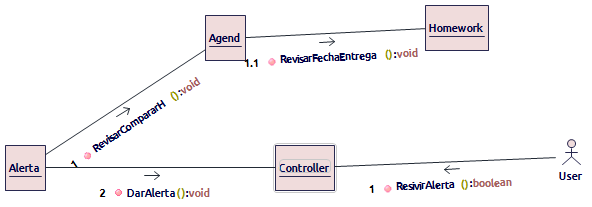
\includegraphics[width=0.7\linewidth]{diseno/requerimientos/imagenes/comunicacion4}
	\caption{Diagrama de comunicación caso de uso 19.}
	\label{fig:gantt}
\end{figure}

Las siguientes tablas, son la especificación de los requerimientos que se considera que tienen un nivel de importancia alta.

 % 1.
\begin{table}[htb]
\centering
\begin{tabular}{|l|c|p{8cm}|}
\hline
RF-01 & \multicolumn {2}{p{10cm}|} {Añadir una tarea }    \\
\hline
Descripción & \multicolumn {2}{p{10cm}|} {El usuario añade una tarea pendiente por desarrollar. }\\
\hline
Precondición & \multicolumn {2}{p{10cm}|} {El usuario debe tener un horario}\\
\cline{2-3}
Secuencia & Paso & Acción \\
\cline{2-3}
& 1 & El usuario selecciona la opción de crear tarea.\\
\cline{2-3}
& 2 & El usuario proporciona la información requerida (nombre de la tarea, tipo, materia a la que pertenece) \\
& 3 & El usuario verifica la información registrada. \\
& 4 & El usuario hace selecciona el botón aceptar. \\
\hline
Postcondición & \multicolumn {2}{p{10cm}|} {El sistema muestra la tarea recién asignada con sus especificaciones y su recomendación de tiempo de realización y de horario } \\
\hline
Excepciones & Paso & Acción \\
\cline{2-3}
& 4 & Se  añade una tarea que requiere urgencia (Imprevisto). El usuario elige que horario sacrificará para realizar la tarea. \\
\cline{2-3}
& 4 & Se añade una tarea que es imposible de realizar debido al tiempo u horario. Es necesario modificar los tiempos u horarios en los que se realizará la tarea o elegir si sacrificar una frnaja de horario. \\
\hline
Rendimiento & Paso & Cota de tiempo \\
\cline{2-3}
& 1 & 1 segundo \\
\cline{2-3}
& 2 & 40 segundos \\
\cline{2-3}
& 3 & 5  segundos \\
\cline{2-3}
& 4 & 1 segundo \\
\hline
Importancia & \multicolumn {2}{p{10cm}|} {Muy importante}    \\
\hline
Urgencia & \multicolumn {2}{p{10cm}|} {urgente}    \\
\hline

\end{tabular}
\end{table}

% 2.
\begin{table}[htb]
\centering
\begin{tabular}{|l|c|p{8cm}|}
\hline
RF-02 & \multicolumn {2}{p{10cm}|} {Añadir subtareas para una tarea. }    \\
\hline
Descripcion & \multicolumn {2}{p{10cm}|} {Se añade una subtarea a una tarea.}\\
\hline
Precondición & \multicolumn {2}{p{10cm}|} {Debe existir alguna tarea pendiente.}\\
\cline{2-3}
Secuencia & Paso & Acción \\
\cline{2-3}
& 1 & El usuario selecciona la tarea a la que desea añadirle una subtarea. \\
\cline{2-3}
& 2 & Seleccionar la opción de añadir subtarea. \\
\cline{2-3}
& 3 & Se añade la subtarea como una tarea (RF-01) \\
\cline{2-3}
& 4 & El usuario verifica la información. \\
\cline{2-3}
& 5 & El pulsa la opción de aceptar.
\hline
Postcondición & \multicolumn {2}{p{10cm}|} {El sistema añadirá la subtarea a la tarea, mostrará sus especificaciones y recomendación de tiempo de realización y de horario} \\
\hline
Excepciones & Paso & Acción \\
\cline{2-3}
& 1 & No existe una tarea para añadirle una subtarea.  \\
\cline{2-3}
& 3 & La subtarea es de carácter urgente.
 \\
\cline{2-3}
& 4 & Se añade una subtarea y esta hace que la tarea sea imposible de terminar debido al tiempo u horario. \\

\hline
Rendimiento & Paso & Cota de tiempo \\
\cline{2-3}
& 1 & 5 segundos \\
\cline{2-3}
& 2 & 1 segundo \\
\cline{2-3}
& 3 & 40 segundos \\
\cline{2-3}
& 4 & 5 segundos  \\
\cline{2-3}
& 5 & 1 segundo \\
\hline
Importancia & \multicolumn {2}{p{10cm}|} {Importante}    \\
\hline
Urgencia & \multicolumn {2}{p{10cm}|} {No urgente}    \\
\hline
Comentarios & No. & Descripción \\
\cline{2-3}
& 1 & Añadir una subtarea es lo mismo que añadir una tarea, la deferencia es que está anidada dentro de una tarea general. 
\hline
\end{tabular}
\end{table}

% 3.
\begin{table}[htb]
\centering
\begin{tabular}{|l|c|p{8cm}|}
\hline
RF- & \multicolumn {2}{p{10cm}|} {Nombre del requisito funcional una vaina asi bien larga carajo pero que no se pase jajajaj }    \\
\hline
Descripcion & \multicolumn {2}{p{10cm}|} {la descripcion}\\
\hline
Precondición & \multicolumn {2}{p{10cm}|} {la precondicion}\\
\cline{2-3}
Secuencia & Paso & Acción \\
\cline{2-3}
& 1 & relatar acción \\
\cline{2-3}
& 2 & relatar acción 2 \\
\hline
Postcondición & \multicolumn {2}{p{10cm}|} {la postcondición} \\
\hline
Excepciones & Paso & Acción \\
\cline{2-3}
& 1 & relatar acción haber probando si se pasa bien o se pasa mal espero que  sea bien jajajaja  \\
\cline{2-3}
& 2 & relatar acción 2 \\
\hline
Rendimiento & Paso & Cota de tiempo \\
\cline{2-3}
& 1 & cota de tiempo 1 \\
\cline{2-3}
& 2 & cota de tiempo 2 \\
\hline
Importancia & \multicolumn {2}{p{10cm}|} {la importancia}    \\
\hline
Urgencia & \multicolumn {2}{p{10cm}|} {la urgencia}    \\
\hline
Comentarios & No. & Descripción \\
\cline{2-3}
& 1 & comentario 1 \\
\cline{2-3}
& 2 & comentario 2 \\
\hline
\end{tabular}
\end{table}

% 4.
\begin{table}[htb]
\centering
\begin{tabular}{|l|c|p{8cm}|}
\hline
RF- & \multicolumn {2}{p{10cm}|} {Nombre del requisito funcional una vaina asi bien larga carajo pero que no se pase jajajaj }    \\
\hline
Descripcion & \multicolumn {2}{p{10cm}|} {la descripcion}\\
\hline
Precondición & \multicolumn {2}{p{10cm}|} {la precondicion}\\
\cline{2-3}
Secuencia & Paso & Acción \\
\cline{2-3}
& 1 & relatar acción \\
\cline{2-3}
& 2 & relatar acción 2 \\
\hline
Postcondición & \multicolumn {2}{p{10cm}|} {la postcondición} \\
\hline
Excepciones & Paso & Acción \\
\cline{2-3}
& 1 & relatar acción haber probando si se pasa bien o se pasa mal espero que  sea bien jajajaja  \\
\cline{2-3}
& 2 & relatar acción 2 \\
\hline
Rendimiento & Paso & Cota de tiempo \\
\cline{2-3}
& 1 & cota de tiempo 1 \\
\cline{2-3}
& 2 & cota de tiempo 2 \\
\hline
Importancia & \multicolumn {2}{p{10cm}|} {la importancia}    \\
\hline
Urgencia & \multicolumn {2}{p{10cm}|} {la urgencia}    \\
\hline
Comentarios & No. & Descripción \\
\cline{2-3}
& 1 & comentario 1 \\
\cline{2-3}
& 2 & comentario 2 \\
\hline
\end{tabular}
\end{table}

% 5.
\begin{table}[htb]
\centering
\begin{tabular}{|l|c|p{8cm}|}
\hline
RF- & \multicolumn {2}{p{10cm}|} {Nombre del requisito funcional una vaina asi bien larga carajo pero que no se pase jajajaj }    \\
\hline
Descripcion & \multicolumn {2}{p{10cm}|} {la descripcion}\\
\hline
Precondición & \multicolumn {2}{p{10cm}|} {la precondicion}\\
\cline{2-3}
Secuencia & Paso & Acción \\
\cline{2-3}
& 1 & relatar acción \\
\cline{2-3}
& 2 & relatar acción 2 \\
\hline
Postcondición & \multicolumn {2}{p{10cm}|} {la postcondición} \\
\hline
Excepciones & Paso & Acción \\
\cline{2-3}
& 1 & relatar acción haber probando si se pasa bien o se pasa mal espero que  sea bien jajajaja  \\
\cline{2-3}
& 2 & relatar acción 2 \\
\hline
Rendimiento & Paso & Cota de tiempo \\
\cline{2-3}
& 1 & cota de tiempo 1 \\
\cline{2-3}
& 2 & cota de tiempo 2 \\
\hline
Importancia & \multicolumn {2}{p{10cm}|} {la importancia}    \\
\hline
Urgencia & \multicolumn {2}{p{10cm}|} {la urgencia}    \\
\hline
Comentarios & No. & Descripción \\
\cline{2-3}
& 1 & comentario 1 \\
\cline{2-3}
& 2 & comentario 2 \\
\hline
\end{tabular}
\end{table}

% 6.
\begin{table}[htb]
\centering
\begin{tabular}{|l|c|p{8cm}|}
\hline
RF- & \multicolumn {2}{p{10cm}|} {Nombre del requisito funcional una vaina asi bien larga carajo pero que no se pase jajajaj }    \\
\hline
Descripcion & \multicolumn {2}{p{10cm}|} {la descripcion}\\
\hline
Precondición & \multicolumn {2}{p{10cm}|} {la precondicion}\\
\cline{2-3}
Secuencia & Paso & Acción \\
\cline{2-3}
& 1 & relatar acción \\
\cline{2-3}
& 2 & relatar acción 2 \\
\hline
Postcondición & \multicolumn {2}{p{10cm}|} {la postcondición} \\
\hline
Excepciones & Paso & Acción \\
\cline{2-3}
& 1 & relatar acción haber probando si se pasa bien o se pasa mal espero que  sea bien jajajaja  \\
\cline{2-3}
& 2 & relatar acción 2 \\
\hline
Rendimiento & Paso & Cota de tiempo \\
\cline{2-3}
& 1 & cota de tiempo 1 \\
\cline{2-3}
& 2 & cota de tiempo 2 \\
\hline
Importancia & \multicolumn {2}{p{10cm}|} {la importancia}    \\
\hline
Urgencia & \multicolumn {2}{p{10cm}|} {la urgencia}    \\
\hline
Comentarios & No. & Descripción \\
\cline{2-3}
& 1 & comentario 1 \\
\cline{2-3}
& 2 & comentario 2 \\
\hline
\end{tabular}
\end{table}

% 7.
\begin{table}[htb]
\centering
\begin{tabular}{|l|c|p{8cm}|}
\hline
RF- & \multicolumn {2}{p{10cm}|} {Nombre del requisito funcional una vaina asi bien larga carajo pero que no se pase jajajaj }    \\
\hline
Descripcion & \multicolumn {2}{p{10cm}|} {la descripcion}\\
\hline
Precondición & \multicolumn {2}{p{10cm}|} {la precondicion}\\
\cline{2-3}
Secuencia & Paso & Acción \\
\cline{2-3}
& 1 & relatar acción \\
\cline{2-3}
& 2 & relatar acción 2 \\
\hline
Postcondición & \multicolumn {2}{p{10cm}|} {la postcondición} \\
\hline
Excepciones & Paso & Acción \\
\cline{2-3}
& 1 & relatar acción haber probando si se pasa bien o se pasa mal espero que  sea bien jajajaja  \\
\cline{2-3}
& 2 & relatar acción 2 \\
\hline
Rendimiento & Paso & Cota de tiempo \\
\cline{2-3}
& 1 & cota de tiempo 1 \\
\cline{2-3}
& 2 & cota de tiempo 2 \\
\hline
Importancia & \multicolumn {2}{p{10cm}|} {la importancia}    \\
\hline
Urgencia & \multicolumn {2}{p{10cm}|} {la urgencia}    \\
\hline
Comentarios & No. & Descripción \\
\cline{2-3}
& 1 & comentario 1 \\
\cline{2-3}
& 2 & comentario 2 \\
\hline
\end{tabular}
\end{table}

% 8.
\begin{table}[htb]
\centering
\begin{tabular}{|l|c|p{8cm}|}
\hline
RF- & \multicolumn {2}{p{10cm}|} {Nombre del requisito funcional una vaina asi bien larga carajo pero que no se pase jajajaj }    \\
\hline
Descripcion & \multicolumn {2}{p{10cm}|} {la descripcion}\\
\hline
Precondición & \multicolumn {2}{p{10cm}|} {la precondicion}\\
\cline{2-3}
Secuencia & Paso & Acción \\
\cline{2-3}
& 1 & relatar acción \\
\cline{2-3}
& 2 & relatar acción 2 \\
\hline
Postcondición & \multicolumn {2}{p{10cm}|} {la postcondición} \\
\hline
Excepciones & Paso & Acción \\
\cline{2-3}
& 1 & relatar acción haber probando si se pasa bien o se pasa mal espero que  sea bien jajajaja  \\
\cline{2-3}
& 2 & relatar acción 2 \\
\hline
Rendimiento & Paso & Cota de tiempo \\
\cline{2-3}
& 1 & cota de tiempo 1 \\
\cline{2-3}
& 2 & cota de tiempo 2 \\
\hline
Importancia & \multicolumn {2}{p{10cm}|} {la importancia}    \\
\hline
Urgencia & \multicolumn {2}{p{10cm}|} {la urgencia}    \\
\hline
Comentarios & No. & Descripción \\
\cline{2-3}
& 1 & comentario 1 \\
\cline{2-3}
& 2 & comentario 2 \\
\hline
\end{tabular}
\end{table}

% 9.
\begin{table}[htb]
\centering
\begin{tabular}{|l|c|p{8cm}|}
\hline
RF- & \multicolumn {2}{p{10cm}|} {Nombre del requisito funcional una vaina asi bien larga carajo pero que no se pase jajajaj }    \\
\hline
Descripcion & \multicolumn {2}{p{10cm}|} {la descripcion}\\
\hline
Precondición & \multicolumn {2}{p{10cm}|} {la precondicion}\\
\cline{2-3}
Secuencia & Paso & Acción \\
\cline{2-3}
& 1 & relatar acción \\
\cline{2-3}
& 2 & relatar acción 2 \\
\hline
Postcondición & \multicolumn {2}{p{10cm}|} {la postcondición} \\
\hline
Excepciones & Paso & Acción \\
\cline{2-3}
& 1 & relatar acción haber probando si se pasa bien o se pasa mal espero que  sea bien jajajaja  \\
\cline{2-3}
& 2 & relatar acción 2 \\
\hline
Rendimiento & Paso & Cota de tiempo \\
\cline{2-3}
& 1 & cota de tiempo 1 \\
\cline{2-3}
& 2 & cota de tiempo 2 \\
\hline
Importancia & \multicolumn {2}{p{10cm}|} {la importancia}    \\
\hline
Urgencia & \multicolumn {2}{p{10cm}|} {la urgencia}    \\
\hline
Comentarios & No. & Descripción \\
\cline{2-3}
& 1 & comentario 1 \\
\cline{2-3}
& 2 & comentario 2 \\
\hline
\end{tabular}
\end{table}

% 10.
\begin{table}[htb]
\centering
\begin{tabular}{|l|c|p{8cm}|}
\hline
RF- & \multicolumn {2}{p{10cm}|} {Nombre del requisito funcional una vaina asi bien larga carajo pero que no se pase jajajaj }    \\
\hline
Descripcion & \multicolumn {2}{p{10cm}|} {la descripcion}\\
\hline
Precondición & \multicolumn {2}{p{10cm}|} {la precondicion}\\
\cline{2-3}
Secuencia & Paso & Acción \\
\cline{2-3}
& 1 & relatar acción \\
\cline{2-3}
& 2 & relatar acción 2 \\
\hline
Postcondición & \multicolumn {2}{p{10cm}|} {la postcondición} \\
\hline
Excepciones & Paso & Acción \\
\cline{2-3}
& 1 & relatar acción haber probando si se pasa bien o se pasa mal espero que  sea bien jajajaja  \\
\cline{2-3}
& 2 & relatar acción 2 \\
\hline
Rendimiento & Paso & Cota de tiempo \\
\cline{2-3}
& 1 & cota de tiempo 1 \\
\cline{2-3}
& 2 & cota de tiempo 2 \\
\hline
Importancia & \multicolumn {2}{p{10cm}|} {la importancia}    \\
\hline
Urgencia & \multicolumn {2}{p{10cm}|} {la urgencia}    \\
\hline
Comentarios & No. & Descripción \\
\cline{2-3}
& 1 & comentario 1 \\
\cline{2-3}
& 2 & comentario 2 \\
\hline
\end{tabular}
\end{table}

% 11.
\begin{table}[htb]
\centering
\begin{tabular}{|l|c|p{8cm}|}
\hline
RF- & \multicolumn {2}{p{10cm}|} {Nombre del requisito funcional una vaina asi bien larga carajo pero que no se pase jajajaj }    \\
\hline
Descripcion & \multicolumn {2}{p{10cm}|} {la descripcion}\\
\hline
Precondición & \multicolumn {2}{p{10cm}|} {la precondicion}\\
\cline{2-3}
Secuencia & Paso & Acción \\
\cline{2-3}
& 1 & relatar acción \\
\cline{2-3}
& 2 & relatar acción 2 \\
\hline
Postcondición & \multicolumn {2}{p{10cm}|} {la postcondición} \\
\hline
Excepciones & Paso & Acción \\
\cline{2-3}
& 1 & relatar acción haber probando si se pasa bien o se pasa mal espero que  sea bien jajajaja  \\
\cline{2-3}
& 2 & relatar acción 2 \\
\hline
Rendimiento & Paso & Cota de tiempo \\
\cline{2-3}
& 1 & cota de tiempo 1 \\
\cline{2-3}
& 2 & cota de tiempo 2 \\
\hline
Importancia & \multicolumn {2}{p{10cm}|} {la importancia}    \\
\hline
Urgencia & \multicolumn {2}{p{10cm}|} {la urgencia}    \\
\hline
Comentarios & No. & Descripción \\
\cline{2-3}
& 1 & comentario 1 \\
\cline{2-3}
& 2 & comentario 2 \\
\hline
\end{tabular}
\end{table}

% 12.
\begin{table}[htb]
\centering
\begin{tabular}{|l|c|p{8cm}|}
\hline
RF- & \multicolumn {2}{p{10cm}|} {Nombre del requisito funcional una vaina asi bien larga carajo pero que no se pase jajajaj }    \\
\hline
Descripcion & \multicolumn {2}{p{10cm}|} {la descripcion}\\
\hline
Precondición & \multicolumn {2}{p{10cm}|} {la precondicion}\\
\cline{2-3}
Secuencia & Paso & Acción \\
\cline{2-3}
& 1 & relatar acción \\
\cline{2-3}
& 2 & relatar acción 2 \\
\hline
Postcondición & \multicolumn {2}{p{10cm}|} {la postcondición} \\
\hline
Excepciones & Paso & Acción \\
\cline{2-3}
& 1 & relatar acción haber probando si se pasa bien o se pasa mal espero que  sea bien jajajaja  \\
\cline{2-3}
& 2 & relatar acción 2 \\
\hline
Rendimiento & Paso & Cota de tiempo \\
\cline{2-3}
& 1 & cota de tiempo 1 \\
\cline{2-3}
& 2 & cota de tiempo 2 \\
\hline
Importancia & \multicolumn {2}{p{10cm}|} {la importancia}    \\
\hline
Urgencia & \multicolumn {2}{p{10cm}|} {la urgencia}    \\
\hline
Comentarios & No. & Descripción \\
\cline{2-3}
& 1 & comentario 1 \\
\cline{2-3}
& 2 & comentario 2 \\
\hline
\end{tabular}
\end{table}

% 13.
\begin{table}[htb]
\centering
\begin{tabular}{|l|c|p{8cm}|}
\hline
RF- & \multicolumn {2}{p{10cm}|} {Nombre del requisito funcional una vaina asi bien larga carajo pero que no se pase jajajaj }    \\
\hline
Descripcion & \multicolumn {2}{p{10cm}|} {la descripcion}\\
\hline
Precondición & \multicolumn {2}{p{10cm}|} {la precondicion}\\
\cline{2-3}
Secuencia & Paso & Acción \\
\cline{2-3}
& 1 & relatar acción \\
\cline{2-3}
& 2 & relatar acción 2 \\
\hline
Postcondición & \multicolumn {2}{p{10cm}|} {la postcondición} \\
\hline
Excepciones & Paso & Acción \\
\cline{2-3}
& 1 & relatar acción haber probando si se pasa bien o se pasa mal espero que  sea bien jajajaja  \\
\cline{2-3}
& 2 & relatar acción 2 \\
\hline
Rendimiento & Paso & Cota de tiempo \\
\cline{2-3}
& 1 & cota de tiempo 1 \\
\cline{2-3}
& 2 & cota de tiempo 2 \\
\hline
Importancia & \multicolumn {2}{p{10cm}|} {la importancia}    \\
\hline
Urgencia & \multicolumn {2}{p{10cm}|} {la urgencia}    \\
\hline
Comentarios & No. & Descripción \\
\cline{2-3}
& 1 & comentario 1 \\
\cline{2-3}
& 2 & comentario 2 \\
\hline
\end{tabular}
\end{table}

% 14.
\begin{table}[htb]
\centering
\begin{tabular}{|l|c|p{8cm}|}
\hline
RF- & \multicolumn {2}{p{10cm}|} {Nombre del requisito funcional una vaina asi bien larga carajo pero que no se pase jajajaj }    \\
\hline
Descripcion & \multicolumn {2}{p{10cm}|} {la descripcion}\\
\hline
Precondición & \multicolumn {2}{p{10cm}|} {la precondicion}\\
\cline{2-3}
Secuencia & Paso & Acción \\
\cline{2-3}
& 1 & relatar acción \\
\cline{2-3}
& 2 & relatar acción 2 \\
\hline
Postcondición & \multicolumn {2}{p{10cm}|} {la postcondición} \\
\hline
Excepciones & Paso & Acción \\
\cline{2-3}
& 1 & relatar acción haber probando si se pasa bien o se pasa mal espero que  sea bien jajajaja  \\
\cline{2-3}
& 2 & relatar acción 2 \\
\hline
Rendimiento & Paso & Cota de tiempo \\
\cline{2-3}
& 1 & cota de tiempo 1 \\
\cline{2-3}
& 2 & cota de tiempo 2 \\
\hline
Importancia & \multicolumn {2}{p{10cm}|} {la importancia}    \\
\hline
Urgencia & \multicolumn {2}{p{10cm}|} {la urgencia}    \\
\hline
Comentarios & No. & Descripción \\
\cline{2-3}
& 1 & comentario 1 \\
\cline{2-3}
& 2 & comentario 2 \\
\hline
\end{tabular}
\end{table}

% 15.
\begin{table}[htb]
\centering
\begin{tabular}{|l|c|p{8cm}|}
\hline
RF- & \multicolumn {2}{p{10cm}|} {Nombre del requisito funcional una vaina asi bien larga carajo pero que no se pase jajajaj }    \\
\hline
Descripcion & \multicolumn {2}{p{10cm}|} {la descripcion}\\
\hline
Precondición & \multicolumn {2}{p{10cm}|} {la precondicion}\\
\cline{2-3}
Secuencia & Paso & Acción \\
\cline{2-3}
& 1 & relatar acción \\
\cline{2-3}
& 2 & relatar acción 2 \\
\hline
Postcondición & \multicolumn {2}{p{10cm}|} {la postcondición} \\
\hline
Excepciones & Paso & Acción \\
\cline{2-3}
& 1 & relatar acción haber probando si se pasa bien o se pasa mal espero que  sea bien jajajaja  \\
\cline{2-3}
& 2 & relatar acción 2 \\
\hline
Rendimiento & Paso & Cota de tiempo \\
\cline{2-3}
& 1 & cota de tiempo 1 \\
\cline{2-3}
& 2 & cota de tiempo 2 \\
\hline
Importancia & \multicolumn {2}{p{10cm}|} {la importancia}    \\
\hline
Urgencia & \multicolumn {2}{p{10cm}|} {la urgencia}    \\
\hline
Comentarios & No. & Descripción \\
\cline{2-3}
& 1 & comentario 1 \\
\cline{2-3}
& 2 & comentario 2 \\
\hline
\end{tabular}
\end{table}

% 16.
\begin{table}[htb]
\centering
\begin{tabular}{|l|c|p{8cm}|}
\hline
RF- & \multicolumn {2}{p{10cm}|} {Nombre del requisito funcional una vaina asi bien larga carajo pero que no se pase jajajaj }    \\
\hline
Descripcion & \multicolumn {2}{p{10cm}|} {la descripcion}\\
\hline
Precondición & \multicolumn {2}{p{10cm}|} {la precondicion}\\
\cline{2-3}
Secuencia & Paso & Acción \\
\cline{2-3}
& 1 & relatar acción \\
\cline{2-3}
& 2 & relatar acción 2 \\
\hline
Postcondición & \multicolumn {2}{p{10cm}|} {la postcondición} \\
\hline
Excepciones & Paso & Acción \\
\cline{2-3}
& 1 & relatar acción haber probando si se pasa bien o se pasa mal espero que  sea bien jajajaja  \\
\cline{2-3}
& 2 & relatar acción 2 \\
\hline
Rendimiento & Paso & Cota de tiempo \\
\cline{2-3}
& 1 & cota de tiempo 1 \\
\cline{2-3}
& 2 & cota de tiempo 2 \\
\hline
Importancia & \multicolumn {2}{p{10cm}|} {la importancia}    \\
\hline
Urgencia & \multicolumn {2}{p{10cm}|} {la urgencia}    \\
\hline
Comentarios & No. & Descripción \\
\cline{2-3}
& 1 & comentario 1 \\
\cline{2-3}
& 2 & comentario 2 \\
\hline
\end{tabular}
\end{table}

% 17.
\begin{table}[htb]
\centering
\begin{tabular}{|l|c|p{8cm}|}
\hline
RF- & \multicolumn {2}{p{10cm}|} {Nombre del requisito funcional una vaina asi bien larga carajo pero que no se pase jajajaj }    \\
\hline
Descripcion & \multicolumn {2}{p{10cm}|} {la descripcion}\\
\hline
Precondición & \multicolumn {2}{p{10cm}|} {la precondicion}\\
\cline{2-3}
Secuencia & Paso & Acción \\
\cline{2-3}
& 1 & relatar acción \\
\cline{2-3}
& 2 & relatar acción 2 \\
\hline
Postcondición & \multicolumn {2}{p{10cm}|} {la postcondición} \\
\hline
Excepciones & Paso & Acción \\
\cline{2-3}
& 1 & relatar acción haber probando si se pasa bien o se pasa mal espero que  sea bien jajajaja  \\
\cline{2-3}
& 2 & relatar acción 2 \\
\hline
Rendimiento & Paso & Cota de tiempo \\
\cline{2-3}
& 1 & cota de tiempo 1 \\
\cline{2-3}
& 2 & cota de tiempo 2 \\
\hline
Importancia & \multicolumn {2}{p{10cm}|} {la importancia}    \\
\hline
Urgencia & \multicolumn {2}{p{10cm}|} {la urgencia}    \\
\hline
Comentarios & No. & Descripción \\
\cline{2-3}
& 1 & comentario 1 \\
\cline{2-3}
& 2 & comentario 2 \\
\hline
\end{tabular}
\end{table}

% 18.
\begin{table}[htb]
\centering
\begin{tabular}{|l|c|p{8cm}|}
\hline
RF- & \multicolumn {2}{p{10cm}|} {Nombre del requisito funcional una vaina asi bien larga carajo pero que no se pase jajajaj }    \\
\hline
Descripcion & \multicolumn {2}{p{10cm}|} {la descripcion}\\
\hline
Precondición & \multicolumn {2}{p{10cm}|} {la precondicion}\\
\cline{2-3}
Secuencia & Paso & Acción \\
\cline{2-3}
& 1 & relatar acción \\
\cline{2-3}
& 2 & relatar acción 2 \\
\hline
Postcondición & \multicolumn {2}{p{10cm}|} {la postcondición} \\
\hline
Excepciones & Paso & Acción \\
\cline{2-3}
& 1 & relatar acción haber probando si se pasa bien o se pasa mal espero que  sea bien jajajaja  \\
\cline{2-3}
& 2 & relatar acción 2 \\
\hline
Rendimiento & Paso & Cota de tiempo \\
\cline{2-3}
& 1 & cota de tiempo 1 \\
\cline{2-3}
& 2 & cota de tiempo 2 \\
\hline
Importancia & \multicolumn {2}{p{10cm}|} {la importancia}    \\
\hline
Urgencia & \multicolumn {2}{p{10cm}|} {la urgencia}    \\
\hline
Comentarios & No. & Descripción \\
\cline{2-3}
& 1 & comentario 1 \\
\cline{2-3}
& 2 & comentario 2 \\
\hline
\end{tabular}
\end{table}

% 19.
\begin{table}[htb]
\centering
\begin{tabular}{|l|c|p{8cm}|}
\hline
RF- & \multicolumn {2}{p{10cm}|} {Nombre del requisito funcional una vaina asi bien larga carajo pero que no se pase jajajaj }    \\
\hline
Descripcion & \multicolumn {2}{p{10cm}|} {la descripcion}\\
\hline
Precondición & \multicolumn {2}{p{10cm}|} {la precondicion}\\
\cline{2-3}
Secuencia & Paso & Acción \\
\cline{2-3}
& 1 & relatar acción \\
\cline{2-3}
& 2 & relatar acción 2 \\
\hline
Postcondición & \multicolumn {2}{p{10cm}|} {la postcondición} \\
\hline
Excepciones & Paso & Acción \\
\cline{2-3}
& 1 & relatar acción haber probando si se pasa bien o se pasa mal espero que  sea bien jajajaja  \\
\cline{2-3}
& 2 & relatar acción 2 \\
\hline
Rendimiento & Paso & Cota de tiempo \\
\cline{2-3}
& 1 & cota de tiempo 1 \\
\cline{2-3}
& 2 & cota de tiempo 2 \\
\hline
Importancia & \multicolumn {2}{p{10cm}|} {la importancia}    \\
\hline
Urgencia & \multicolumn {2}{p{10cm}|} {la urgencia}    \\
\hline
Comentarios & No. & Descripción \\
\cline{2-3}
& 1 & comentario 1 \\
\cline{2-3}
& 2 & comentario 2 \\
\hline
\end{tabular}
\end{table}

% 20.
\begin{table}[htb]
\centering
\begin{tabular}{|l|c|p{8cm}|}
\hline
RF- & \multicolumn {2}{p{10cm}|} {Nombre del requisito funcional una vaina asi bien larga carajo pero que no se pase jajajaj }    \\
\hline
Descripcion & \multicolumn {2}{p{10cm}|} {la descripcion}\\
\hline
Precondición & \multicolumn {2}{p{10cm}|} {la precondicion}\\
\cline{2-3}
Secuencia & Paso & Acción \\
\cline{2-3}
& 1 & relatar acción \\
\cline{2-3}
& 2 & relatar acción 2 \\
\hline
Postcondición & \multicolumn {2}{p{10cm}|} {la postcondición} \\
\hline
Excepciones & Paso & Acción \\
\cline{2-3}
& 1 & relatar acción haber probando si se pasa bien o se pasa mal espero que  sea bien jajajaja  \\
\cline{2-3}
& 2 & relatar acción 2 \\
\hline
Rendimiento & Paso & Cota de tiempo \\
\cline{2-3}
& 1 & cota de tiempo 1 \\
\cline{2-3}
& 2 & cota de tiempo 2 \\
\hline
Importancia & \multicolumn {2}{p{10cm}|} {la importancia}    \\
\hline
Urgencia & \multicolumn {2}{p{10cm}|} {la urgencia}    \\
\hline
Comentarios & No. & Descripción \\
\cline{2-3}
& 1 & comentario 1 \\
\cline{2-3}
& 2 & comentario 2 \\
\hline
\end{tabular}
\end{table}

